Die Funktion
\[
\varphi(x)
=
\begin{cases}
0         &\qquad x\le 0\\
a(x^2-x^4)&\qquad 0< x \le 1\\
0         &\qquad 1<x
\end{cases}
\]
soll als Wahrscheinlichkeitsdichte einer Zufallsvariable $X$ verwendet werden.
\begin{center}
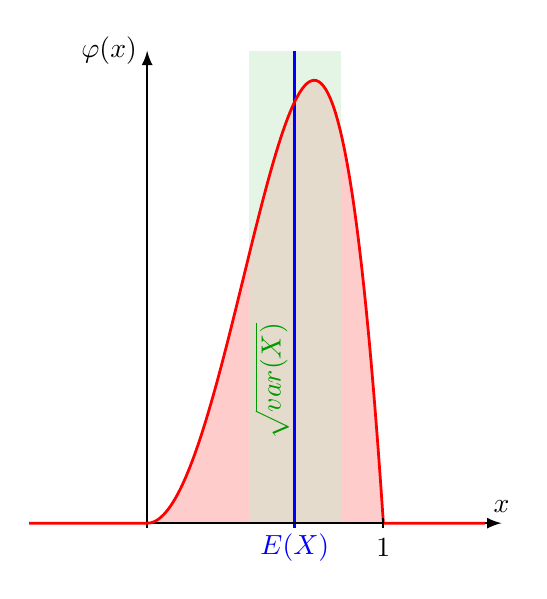
\begin{tikzpicture}[>=latex,thick,scale=3]
\definecolor{darkgreen}{rgb}{0,0.6,0}
\fill[color=red!20]
	plot[domain=0:1,samples=100] ({\x},{(15/2)*(\x*\x*(1-\x*\x))})
	--
	(1,0)
	-- cycle;
\ifthenelse{\boolean{pruefung}}{}{
\fill[color=darkgreen!20,opacity=0.5]
	({5/8-sqrt(17/448)},0) rectangle ({5/8+sqrt(17/448)},2);
\node[color=darkgreen] at ({5/8-0.5*sqrt(17/448)},0.6)
	[rotate=90] {$\sqrt{\operatorname{var}(X)}$};
\draw[line width=1pt,color=blue] ({5/8},-0.02) -- ({5/8},2);
\node[color=blue] at ({5/8},0) [below] {$E(X)$};
}
\draw[->] (-0.5,0) -- (1.5,0) coordinate[label={$x$}];
\draw[->] (0,-0.02) -- (0,2.0) coordinate[label={left:$\varphi(x)$}];
\draw[color=red,line width=1pt] (-0.5,0)
	--
	plot[domain=0:1,samples=100] ({\x},{(15/2)*(\x*\x*(1-\x*\x))})
	--
	(1,0)
	--
	(1.43,0);
\draw (1,-0.02) -- (1,0.02);
\node at (1,-0.02) [below] {$1$};
\end{tikzpicture}
\end{center}
\begin{teilaufgaben}
\item
Wie muss $a$ gewählt werden, damit $\varphi(x)$ tatsächlich eine
Wahrscheinlichkeitsdichte sein kann?
\item
Bestimmen Sie den Erwartungswert von $X$.
\item
Bestimmen Sie die Verteilungsfunktion $F_X(x)$.
\item
Bestimmen Sie die Varianz von $X$.
\item
\label{50000043:median}
Bestimmen Sie den Median von $X$.
\end{teilaufgaben}

\thema{Wahrscheinlichkeitsdichte}
\thema{Verteilungsfunktion}
\thema{Erwartungswert}
\thema{Varianz}

\begin{loesung}
\begin{teilaufgaben}
\item
$a$ muss so gewählt werden, dass das Integral von $\varphi$ über
$\mathbb R$ den Wert $1$ haben muss.
Man berechnet daher
\begin{align*}
\int_{-\infty}^\infty \varphi(x)\,dx
&=
\int_0^1 a(x^2-x^4)\,dx
=
a \biggl[ \frac{x^3}3 - \frac{x^5}5 \biggr]_0^1
=
a\biggl(\frac13-0-\frac15+0\biggr)
=
a\frac{5-3}{15}
=
\frac{2a}{15}
=
1
\\
\Rightarrow\qquad
a
&=
\frac{15}{2}.
\end{align*}
\item
Der Erwartungswert ist das Integral von $x\varphi(x)$:
\begin{align*}
E(X)
&=
\int_{-\infty}^{\infty} x\, \varphi(x)\,dx
=
\int_0^1 x\cdot a(x^2-x^4)\,dx
=
a \int_0^1 x^3-x^5\,dx
\\
&=
a\biggl[\frac{x^4}{4}-\frac{x^6}6\biggr]_0^1
=
a\biggl( \frac{1}{4} - \frac{1}{6}\biggr)
=
\frac{15}{2} \frac{3-2}{12}
=
\frac{5}{8}.
\end{align*}
\item
Die Verteilungsfunktion ist für $x$-Werte zwischen $0$ und $1$:
\begin{align*}
F_X(x)
&=
\int_{-\infty}^x \varphi(\xi)\,d\xi
=
\int_0^x a(x^2-x^4)\,dx
=
a\biggl[\frac{\xi^3}{3} - \frac{\xi^5}{5}\biggr]_0^x
=
\frac{15}{2} \biggl(\frac{x^3}{3}-\frac{x^5}{5}\biggr)
=
\frac{5x^3-3x^5}{2}
\end{align*}
Die Verteilungsfunktion insgesamt ist damit
\[
F_X(x)
=
\begin{cases}
0&\qquad x\le 0\\
\displaystyle\frac{5x^3-3x^5}{2}&\qquad 0<x\le 1\\
1&\qquad x>1.
\end{cases}
\]
\item
Für die Varianz brauchen wir zunächst den Erwartungswert $E(X^2)$ von $X^2$:
\begin{align*}
E(X^2)
&=
\int_{-\infty}^\infty x^2\,\varphi(x)\,dx
=
\int_0^1 x^2\cdot a(x^2-x^4)\,dx
=
a\int_0^1 x^4-x^6\,dx
\\
&=
a\biggl[ \frac{x^5}{5}-\frac{x^7}{7}\biggr]_0^1
=
a\biggl(\frac{1}{5}-\frac{1}{7}\biggr)
=
\frac{15}{2}\frac{7-5}{5\cdot 7}
=
\frac{3}{7}.
\end{align*}
Daraus kann man jetzt die Varianz bekommen als
\[
\operatorname{var}(X)
=
E(X^2)-E(X)^2
=
\frac{3}{7} - \biggl(\frac{5}{8}\biggr)^2
=
\frac{3}{7}-\frac{25}{64}
=
\frac{17}{448}
\approx
0.037946.
\]
\item
Der Median $x_{\text{med}}$ ist derjenige Wert, für den
$F_X(x_{\text{med}}) = \frac12$ ist.
Es gilt also
\begin{align*}
\frac{5x_{\text{med}}^3-3x_{\text{med}}^5}{2} &= \frac12 \\
3x_{\text{med}}^5-5x_{\text{med}}^3+1&=0
&&\Rightarrow&
x_{\text{med}} &= 0.64313878216335.
\end{align*}
Diese Gleichung fünften Grades kann nur numerisch gelöst werden.
\qedhere
\end{teilaufgaben}
\end{loesung}

%\begin{diskussion}
%Teilaufgabe~e) war nicht Teil der Prüfung.
%\end{diskussion}
\begin{bewertung}
\begin{teilaufgaben}
\item Wert von $a$ ({\bf A}) 1 Punkt.
\item Erwartungswert ({\bf E}) 1 Punkt.
\item Verteilungsfunktion ({\bf F}) 1 Punkt.
\item Varianzformel ({\bf V}) 1 Punkt,
Erwartungswert von $X^2$ ({\bf E2}) 1 Punkt.
\item Median ({\bf M}) 1 Punkt.
\end{teilaufgaben}
\end{bewertung}
